% Graphical abstract. Compile from this folder:
%   pdflatex -interaction=nonstopmode -halt-on-error -output-directory=../Figures fig_graphical_abstract.tex
% Include in the graphicalabstract environment:
%   
\includegraphics[width=\linewidth]{Figures/fig_graphical_abstract}
\documentclass[tikz,border=7pt]{standalone}
\usepackage[scaled=0.95]{helvet}
\renewcommand{\familydefault}{\sfdefault}
\usepackage{xcolor}
\usetikzlibrary{arrows.meta,calc,fit,backgrounds}

\definecolor{ink}{HTML}{1F2933}
\definecolor{muted}{HTML}{5B6776}
\definecolor{line}{HTML}{9AA7B5}
\definecolor{panel}{HTML}{F7F9FC}
\definecolor{bluefill}{HTML}{E8EEF5}
\definecolor{greenfill}{HTML}{EAF4EC}
\definecolor{amberfill}{HTML}{FFF4E3}
\definecolor{accent}{HTML}{255E88}

\begin{document}
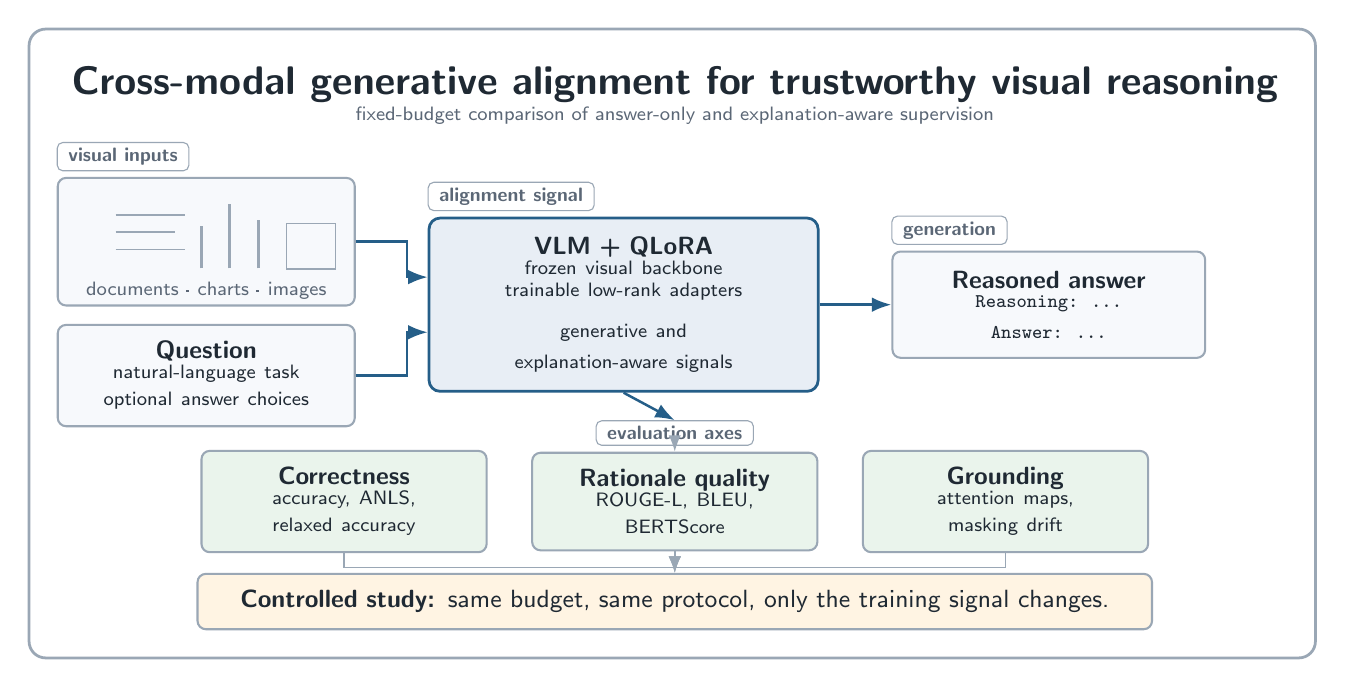
\begin{tikzpicture}[
  font=\sffamily\small,
  >=Latex,
  arrow/.style={->,line width=0.9pt,draw=accent},
  guide/.style={line width=0.65pt,draw=line},
  card/.style={draw=line,fill=panel,rounded corners=3pt,line width=0.75pt,
               inner sep=6pt,align=center,text=ink},
  main/.style={draw=accent,fill=bluefill,rounded corners=4pt,line width=1.0pt,
               inner sep=7pt,align=center,text=ink},
  metric/.style={draw=line,fill=greenfill,rounded corners=3pt,line width=0.75pt,
                 inner sep=6pt,align=center,text=ink},
  note/.style={draw=line,fill=amberfill,rounded corners=3pt,line width=0.75pt,
               inner sep=6pt,align=center,text=ink},
  chip/.style={draw=line,fill=white,rounded corners=2pt,inner xsep=4pt,inner ysep=2pt,
               font=\scriptsize\bfseries,text=muted},
  title/.style={font=\sffamily\Large\bfseries,text=ink},
  subtitle/.style={font=\sffamily\scriptsize,text=muted}
]

% Title
\node[title] (title) at (8.2,7.35)
  {Cross-modal generative alignment for trustworthy visual reasoning};
\node[subtitle] at (8.2,6.95)
  {fixed-budget comparison of answer-only and explanation-aware supervision};

% Left column: inputs
\node[card,text width=3.35cm,minimum height=1.62cm] (visual) at (2.25,5.35) {};
\node[chip,anchor=south west] at ($(visual.north west)+(0,2pt)$) {visual inputs};
\draw[guide] ($(visual.center)+(-1.15,0.34)$) -- ++(0.88,0);
\draw[guide] ($(visual.center)+(-1.15,0.12)$) -- ++(0.75,0);
\draw[guide] ($(visual.center)+(-1.15,-0.10)$) -- ++(0.88,0);
\draw[guide,line width=1.1pt] ($(visual.center)+(-0.06,-0.34)$) -- ++(0,0.54);
\draw[guide,line width=1.1pt] ($(visual.center)+(0.30,-0.34)$) -- ++(0,0.82);
\draw[guide,line width=1.1pt] ($(visual.center)+(0.66,-0.34)$) -- ++(0,0.62);
\draw[guide] ($(visual.center)+(1.02,-0.35)$) rectangle ++(0.62,0.58);
\node[subtitle] at ($(visual.center)+(0,-0.62)$) {documents · charts · images};

\node[card,text width=3.35cm,minimum height=1.0cm] (question) at (2.25,3.65)
  {\textbf{Question}\\[-1pt]\scriptsize natural-language task\\[-1pt]\scriptsize optional answer choices};

% Middle column: method
\node[main,text width=4.45cm,minimum height=2.0cm] (model) at (7.55,4.55)
  {\textbf{VLM + QLoRA}\\[-1pt]
   \scriptsize frozen visual backbone\\
   \scriptsize trainable low-rank adapters\\[4pt]
   \scriptsize generative and explanation-aware signals};
\node[chip,anchor=south west] at ($(model.north west)+(0,2pt)$) {alignment signal};

% Right column: output
\node[card,text width=3.55cm,minimum height=1.35cm] (answer) at (12.95,4.55)
  {\textbf{Reasoned answer}\\[-1pt]
   \scriptsize \texttt{Reasoning: ...}\\
   \scriptsize \texttt{Answer: ...}};
\node[chip,anchor=south west] at ($(answer.north west)+(0,2pt)$) {generation};

% Evaluation row
\node[chip] (measure) at (8.2,2.92) {evaluation axes};
\node[metric,text width=3.2cm,minimum height=1.05cm] (m1) at (4.0,2.05)
  {\textbf{Correctness}\\[-1pt]\scriptsize accuracy, ANLS,\\[-1pt]\scriptsize relaxed accuracy};
\node[metric,text width=3.2cm,minimum height=1.05cm] (m2) at (8.2,2.05)
  {\textbf{Rationale quality}\\[-1pt]\scriptsize ROUGE-L, BLEU,\\[-1pt]\scriptsize BERTScore};
\node[metric,text width=3.2cm,minimum height=1.05cm] (m3) at (12.4,2.05)
  {\textbf{Grounding}\\[-1pt]\scriptsize attention maps,\\[-1pt]\scriptsize masking drift};

\node[note,text width=11.7cm,minimum height=0.68cm] (study) at (8.2,0.78)
  {\textbf{Controlled study:} same budget, same protocol, only the training signal changes.};

% Flow: no crossing arrows
\draw[arrow] (visual.east) -- ++(0.65,0) |- ($(model.west)+(0,0.35)$);
\draw[arrow] (question.east) -- ++(0.65,0) |- ($(model.west)+(0,-0.35)$);
\draw[arrow] (model.east) -- (answer.west);
\draw[arrow] (model.south) -- (measure.north);
\draw[guide,->] (measure.south) -- (m2.north);
\draw[guide,->] (m1.south) -- ++(0,-0.18) -| (study.north);
\draw[guide,->] (m2.south) -- (study.north);
\draw[guide,->] (m3.south) -- ++(0,-0.18) -| (study.north);

\begin{scope}[on background layer]
  \node[draw=line,fill=white,rounded corners=6pt,line width=1.0pt,
        fit=(title)(visual)(question)(model)(answer)(m1)(m3)(study),
        inner sep=10pt] {};
\end{scope}

\end{tikzpicture}
\end{document}
